% Drawn by scripts/revision3/fig_appendix_flows.py; the .pptx is the editable
% source and is released with the paper.
\begin{figure}[t]
\centering
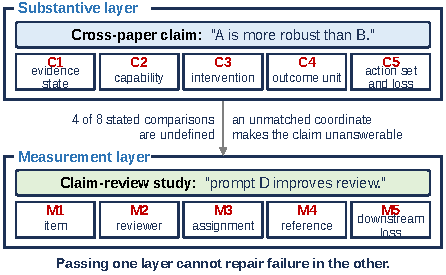
\includegraphics[width=\columnwidth]{figures/generated/fig_two_layer.pdf}%
\caption{The two layers answer different questions about the same sentence.
The substantive layer asks whether two published results concern one decision
problem; Table~\ref{tab:cross-paper-cases} applies it to real comparisons and
supplies the four-of-eight count. The measurement layer asks what a study of
claim review estimates; Table~\ref{tab:retrospective-remedies} shows which
analyses of such a study are valid. Passing one layer cannot repair failure in
the other.}
\label{fig:two-layer}
\end{figure}
